\documentclass[11pt]{beamer}
\mode<presentation>

\usepackage[italian]{babel}
\usepackage{euscript}
\usepackage[utf8]{inputenc}

\usepackage{subfigure}
\usepackage{graphicx}
\usepackage{verbatim}
\usepackage{makeidx}
\pagestyle{empty}
%\usepackage{graphics}
%\usepackage[dvips]{graphicx}
%\usepackage{verbatim}
%\usepackage{subfigure}
%\usepackage{makeidx}
%\usepackage{eurosym}
%\usepackage{amsfonts}
%\usepackage{latexsym}
%\usepackage{makeidx}
%\usepackage{amsmath}
%\usepackage{amsthm}
%\usepackage{comment}
%\usepackage{enumerate}
%\usepackage{mathrsfs}
\pagestyle{empty}

%%%%%%%%%%%%%%%%%%%%%%%%%%% Definizione teoremi: $%%%%%

\newtheorem{definizione}{Definizione}
\newtheorem{esempio}{Esempio}
\newtheorem{osservazione}{Osservazione}
\newtheorem{lemmax}{Lemma}[section]
\newtheorem{teorema}{Teorema}
\newtheorem{prop}{Proprietà}
\newtheorem{corollario}{Corollario}

%%%%%%%%%%%%%%%%%%%%%%%%%%%%%%%%%%%%%%%%%%%

\usetheme{Copenhagen}

%%%%%%%%%%%%%%%%%%%%%%%%%%



\title{Tesi di Laurea}
\author{Sebastiano Ferraris}
\date{}
\subtitle{TRE PROBLEMI IMPOSSIBILI}
\institute{Università degli studi di Torino \\Facoltà di Scienze Matematiche Fisiche Naturali \\ Corso di laurea in Matematica}

\begin{document}


%%%%%%%%%%%%%%%%%%%%%%%%%%%%%%%%%%
%%% 0) TITOLO! %%%%%%%%%%%%%%%%%%%%%%%%%%
\begin{frame}
 \maketitle
\begin{figure}[!h]
\begin{center}
\resizebox{3.0 cm}{3.0 cm}{
\includegraphics{unito.jpg}}
\end{center}
\end{figure}
\end{frame}



%%%%%%%%%%%%%%%%%%%%%%%%%%%%%%%%%%%%%%%%%
%%%%%%%%%%%%%%%%%%%%%%%%%%%%%%%%%%%%%%%%%
%%%%%%%%%%%%%%%%%%%%%%%%%%%%%%%%%%%%%%%%%
%%% 1.1) Intro capitolo 1 %%%%%%%%%%%%%%%%%%%%%%%%%%%%

\begin{frame}
\begin{center}
Capitolo 1 \\
COSTRUZIONI CON RIGA E COMPASSO
\end{center}
\end{frame}


%%%%%%%%%%%%%%%%%%%%%%%%%%%%%%%%%%%%%%%
%%% 1.2) costruzioni euclidee definizioni %%%%%%%%%%%%%%%%%%%%
\begin{frame}
\frametitle{Costruzioni Euclidee: definizione}
\begin{definizione} 
Dato un piano e una distanza fissata $U$, una \begin{bfseries}costruzione euclidea\end{bfseries} è una successione $(K_{0}, K_{1},..., K_{n})$ i cui elementi possono essere punti, rette, o circonferenze nel piano, in modo che:

\begin{enumerate}

\item $K_{0}$ è un punto iniziale e $K_{1}$, un punto a distanza $U$ da $K_{0}$.

\item Se $K_{i}$ per $ 2\le i \le n$ è una retta, allora deve passare per due punti $K_{r}$ $K_{s}$ con $r, s < i$.

\item Se $K_{i}$ per $ 2 \le i \le n$ è una circonferenza, allora ha centro un punto $K_{c}$ e raggio il segmento $K_{r}K_{s}$, con $c, r, s < i$.

\item Se $K_{i}$ per $ 2\le i \le n$ è un punto, allora può essere o punto a distanza fissata $U$ da un altro punto $K_{a}$, oppure può essere un'intersezione fra due circonferenze $K_{b}$, $K_{c}$, fra due rette $K_{d}$, $K_{e}$, o fra una retta ed una circonferenza $K_{f}$, $K_{g}$, con $a,b,c,d,e,f,g < i$. 
\end{enumerate}
\end{definizione}
\end{frame}


%%%%%%%%%%%%%%%%%%%%%%%%%%%%%%%%%%%%%
%%% 1.3) costruzioni euclidee osservazione
\begin{frame}
\frametitle{Costruzioni Euclidee: osservazione sulla notazione}
\begin{osservazione}
Si propone la seguente notazione per i diversi $K_{i}$ della successione: 
\begin{itemize}

\item Se $K_{i}$è uno dei due punti iniziali, allora si ha rispettivamente $K_{0} := P_{0}$ e $K_{1} := P_{1}$.

\item Se $K_{i}$ è una retta fra due punti $P_{r}$ e $P_{s}$, allora $K_{i} := R_{i} (P_{r}, P_{s})$;

\item Se $K_{i}$ è una circonferenza di centro $P_{c}$ e di raggio il segmento avente per estremi i punti $P_{r}$ e $P_{s}$, allora $K_{i} := C_{i} (P_{c}; \overline{P_{r}P_{s}})$;

\item Se $K_{i}$ è un punto di intersezione fra due circonferenze $C_{a}$, $C_{b}$, oppure di due rette $R_{a}$, $R_{b}$, oppure di una retta $R_{a}$ e una circonferenza $C_{b}$, allora si ha rispettivamente $K_{i} := P_{i} (C_{a},C_{b})$, $K_{i} := P_{i} (R_{a},R_{b})$ oppure $K_{i} := P_{i} (R_{a},C_{b})$.

\end{itemize}

\end{osservazione}

\end{frame}


%%%%%%%%%%%%%%%%%%%%%%%%%%%%%%%%%%%%%%
%%% 1.4) costruzioni euclidee Esempi
\begin{frame}
\frametitle{Costruzioni Euclidee: esempi fondamentali}

Con il sistema appena definito è sempre possibile

\begin{itemize}

\item Costruire la retta perpendicolare ad una retta data.

\item Costruire un sistema di assi cartesiani con ripartizioni di segmenti di lunghezza $U$.

\item Costruire la bisettrice di un quadrante.

\item Trovare il punto medio di un segmento.

\item Costruire la retta parallela ad una retta data per un punto dato.

\end{itemize}

\end{frame}


%%%%%%%%%%%%%%%%%%%%%%%%%%%%%%%%%%%%%%%%%
%%% 1.5) costruzioni euclidee Esempio retta parallela
\begin{frame}
\frametitle{Costruzioni Euclidee: costruzione della retta parallela I}
A titolo di esempio, si propone la costruzione della retta parallela ad una retta data per un punto dato:

%%%%%%%% IMMAGINE COSTRUZIONE PARALLELE %
\begin{figure}[!h]
%centrare
\begin{center}
\resizebox{8.5 cm}{6.3 cm}{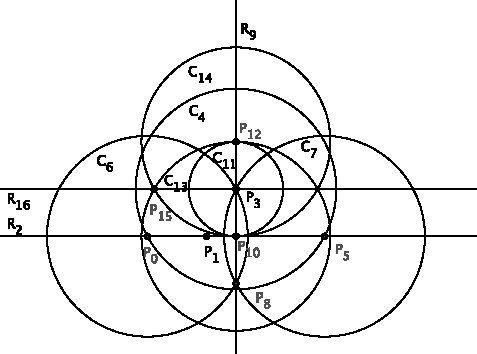
\includegraphics{1_Es5_parall}} 
%\includegraphics{Es1perpendicolare} 
\caption{Rette parallele}
\end{center}
\end{figure}
\end{frame}


%%%%%%%%%%%%%%%%%%%%%%%%%%%%%%%%%%%%%%%%%
%%% 1.5) costruzioni euclidee Esempio retta parallela
\begin{frame}
\frametitle{Costruzioni Euclidee: costruzione della retta parallela II}
... Avvalendosi della notazione introdotta, al diagramma precedente corrisponde la successione:

\begin{align*}
S_{p} = (&P_{0}, P_{1}, R_{2}(P_{0}, P_{1}), P_{3}, C_{4}(P_{3}; \overline{P_{3} P_{0}}), P_{5}(R_{2},C_{4}), C_{6}(P_{0}; \overline{P_{0} P_{3}}), \\
&C_{7}(P_{5}; \overline{P_{5} P_{3}}), P_{8}(C_{6},C_{7}), R_{9}(P_{3}, P_{8}), P_{10}(R_{2},R_{9}), \\
& C_{11}(P_{3}; \overline{P_{3} P_{10}}), P_{12}(R_{9}, C_{11}), C_{13}(P_{10}; \overline{P_{10} P_{12}}), \\
&  C_{14}(P_{12}; \overline{P_{10} P_{12}}),  P_{15}(C_{13},C_{14}), R_{16}(P_{3}, P_{15}) )
\end{align*}
\end{frame}



%%%%%%%%%%%%%%%%%%%%%%%%%%%%%%%%%%%%%% Prima scelta
%%% 1.4) costruzioni euclidee Esempi
\begin{frame}
\frametitle{Costruzioni Euclidee: manipolazione di due segmenti}

Inoltre, dati due segmenti di lunghezza $\alpha$ e $\beta$, è sempre possibile

\begin{itemize}

\item Costruire il segmento di lunghezza $\alpha + \beta$ e $\alpha - \beta$.

\item Costruire il segmento di lunghezza $\alpha \cdot \beta$ e $\alpha / \beta$.

\item Costruire il segmento di lunghezza $\alpha^{-1} $

\item Costruire il segmento di lunghezza $\sqrt{\alpha}$.

\end{itemize}

\end{frame}


%%%%%%%%%%%%%%%%%%%%%%%%%%%%%%%%%%%%%%%%%
%%%%%%%%%%%%%%%%%%%%%%%%%%%%%%%%%%%%%%%%%
%%%%%%%%%%%%%%%%%%%%%%%%%%%%%%%%%%%%%%%%%
%%% 1.1) Intro capitolo 2 %%%%%%%%%%%%%%%%%%%%%%%%%%%%

\begin{frame}
\begin{center}
Capitolo 2 \\
NUMERI EUCLIDEI
\end{center}
\end{frame}


%%%%%%%%%%%%%%%%%%%%%%%%%%%%%%%%%%%%%%%
%%% 2.1) costruzioni euclidee definizioni %%%%%%%%%%%%%%%%%%%%
\begin{frame}
\frametitle{Numeri euclidei: definizioni}

%Sia $\mathcal{E}_{\mathbb{R}\times\mathbb{R}}$ l'insieme delle  \begin{bfseries}costruzioni euclidee nel piano reale\end{bfseries}.
%% def di punti euclidei
\begin{definizione}
Un punto $Q$ di $\mathbb{R}\times\mathbb{R}$ che compare in una \begin{bfseries}costruzioni euclidee nel piano reale\end{bfseries}, è detto \begin{bfseries}punto euclideo\end{bfseries}  o costruibile. L'insieme di tutti i punti euclidei sarà indicato con $E$.
\end{definizione}

%%%%%%%%%%%%%% Numero reale Euclideo
\begin{definizione}
$\gamma \in \mathbb{R}$ è detto \begin{bfseries}numero reale euclideo\end{bfseries} se esiste una costruzione euclidea nel piano reale nella quale compare un segmento di lunghezza $|\gamma|$.
\end{definizione}

%%%%%%%%%%% Numero complesso  Euclideo
\begin{definizione}
$a + i b \in \mathbb{C}$ è detto \begin{bfseries}numero complesso euclideo\end{bfseries} se il corrispondente punto $(a, b) \in \mathbb{R}\times\mathbb{R}$ appartiene ad una costruzione euclidea nel piano reale.
\end{definizione}

\end{frame}



%%%%%%%%%%%%%%%%%%%%%%%%%%%%%%%%%%%%%%%
%%% 1.2) costruzioni euclidee definizioni %%%%%%%%%%%%%%%%%%%%
\begin{frame}
\frametitle{Numeri euclidei: caratterizzazione algebrica di E }

% proprietà di caratterizzazione di E come campo
\begin{prop}
Dato $E$, insieme dei punti euclidei del piano reale, si ha che
\begin{enumerate} [i)]
\item $\mathbb{Z} \subset E$ 
\item $\mathbb{Q} \subset E$
\item $E$ è un campo.
\end{enumerate}
\end{prop}

%osservazione su E come estensione di grado due
\begin{osservazione} 
Dalla possibilità di costruire $\sqrt{\alpha}$ per $\alpha$ segmento già costruito, segue che se un numero $z$ è euclideo allora lo è anche la sua radice quadrata.
\begin{align*}
\forall z \in E \Rightarrow \sqrt{z} \in E
\end{align*}
\end{osservazione}
\end{frame}


%%%%%%%%%%%%%%%%%%%%%%%%%%%%%%%%%%%%%%%
%%%% 1.2) costruzioni euclidee definizioni %%%%%%%%%%%%%%%%%%%%
%\begin{frame}
%\frametitle{Numeri euclidei: E come estensione di $\mathbb{Q}$  }
%Si può affermare che:
%\begin{align*}
%\forall q_0 \in \mathbb{Q} \quad \Rightarrow \quad \sqrt{q_0} \in E \quad \Rightarrow \quad \mathbb{Q}(\sqrt{q_0}) \subset E
%\end{align*}
%\noindent
%dove $\mathbb{Q}(\sqrt{q_0})$ è la più piccola estensione di $\mathbb{Q}$ contenente $\sqrt{q_0}$.

%\noindent
%Ripetendo il ragionamento, si ha che
%\begin{align*}
%\forall q_1 \in \mathbb{Q}(\sqrt{q_0})  \Rightarrow q_1 \in E \Rightarrow \sqrt{q_1} \in E \Rightarrow  \mathbb{Q}(\sqrt{q_0}, \sqrt{q_1}) \subset E
%\end{align*}

%Si può quindi estendere il campo $\mathbb{Q}$ con una successione di radici, ottenendo sempre un sottocampo di $E$. \\
%Inoltre
%\begin{align*}
%[ \mathbb{Q}(\sqrt{q_0},\sqrt{q_1} \dots \sqrt{q_i}): \mathbb{Q}(\sqrt{q_0},\sqrt{q_1} \dots \sqrt{q_{i-1}})] \leq 2 
%\end{align*}

%\end{frame}



%%%%%%%%%%%%%%%%%%%%%%%%%%%%%%%%%%%%%%%
%%% 1.2) costruzioni euclidee definizioni %%%%%%%%%%%%%%%%%%%%
\begin{frame}
\frametitle{Numeri euclidei: conseguenze}

\begin{teorema}[fondamentale]
Un numero complesso $\alpha$ è euclideo se e solo se esiste una successione di campi 
\begin{align*}
\mathbb{Q} = \mathbb{E}_0 \subseteq \mathbb{E}_1 \subseteq ... \subseteq  \mathbb{E}_{n+1}  
\end{align*}
\noindent
tale che $\alpha \in  \mathbb{E}_{n+1}$ ed    $[\mathbb{E}_{j+1}: \mathbb{E}_{j}] \leq 2$ per $j = 0, 1, ... , n $
\end{teorema}

\begin{corollario}
Se $\alpha \in \mathbb{C}$ è euclideo, allora $\alpha$ è algebrico di grado $2^k$ per un opportuno naturale k.
\end{corollario}


\begin{corollario}
Se un numero reale $\beta$ è radice di un polinomio irriducibile di grado $n$ che non è una potenza di $2$, allora $\beta$ non è un numero euclideo.
\end{corollario}

\end{frame}


%%%%%%%%%%%%%%%%%%%%%%%%%%%%%%%%%%%%%%%%%
%%%%%%%%%%%%%%%%%%%%%%%%%%%%%%%%%%%%%%%%%
%%%%%%%%%%%%%%%%%%%%%%%%%%%%%%%%%%%%%%%%%
%%% Intro capitolo 3 %%%%%%%%%%%%%%%%%%%%%%%%%%%%

\begin{frame}
\begin{center}
Capitolo 3 \\ESTENSIONI CICLOTOMICHE
\end{center}
\end{frame}

%%%%%%%%%%%%%%%%%%%%%%%%%%%%%%%%%%%%%%%
%%% 3.1) costruzioni euclidee definizioni %%%%%%%%%%%%%%%%%%%%
\begin{frame}
\frametitle{Estensioni ciclotomiche: introduzione}
\begin{center}
Per quali $n \in \mathbb{N}$ è possibile costruire il poligono regolare di $n$ lati con riga e compasso?
\end{center}
%%%%%% Osservazione radici n-esime
\begin{osservazione}
Il problema è equivalente a quello di costruire le soluzioni di $x^n - 1 = 0$. Infatti tale equazione polinomiale ha esattamente $n$ soluzioni distinte nel piano di Gauss: 
\begin{align*} 
\delta_{n}^{k} := e^{\frac{2k\pi i}{n}} = \cos(\frac{2k\pi i}{n}) + i \sin(\frac{2k\pi i}{n})  \quad k = 0 \dots n-1
\end{align*}
\end{osservazione}
\begin{center}
Per tutti gli $n$ tali che il numero complesso $\delta_{n}^{1}$ è euclideo.
\end{center}
\end{frame}




%%%%%%%%%%%%%%%%%%%%%%%%%%%%%%%%%%%%%%%
%%% 3.2) costruzioni euclidee definizioni %%%%%%%%%%%%%%%%%%%%
\begin{frame}
\frametitle{Estensioni ciclotomiche: definizioni}

\begin{definizione}
Una radice $n$-esima dell'unità $\delta_{n}^{k}$ si dice \begin{bfseries}primitiva\end{bfseries}, se $(\delta_{n}^{k})^n = 1$. 
\end{definizione}

\begin{center}
Ci sono esattamente $\phi(n)$ radici $n$-esime primitive dell'unità.
\end{center}

\begin{definizione} 
Il campo di spezzamento del polinomio $x^n - 1$ su $\mathbb{Q}$ è detto \begin{bfseries}estensione ciclotomica\end{bfseries}. 
\end{definizione}

\begin{center}
Dato che ci sono esattamente $\phi(n)$ radici $n$-esime primitive dell'unità, l'estensione ciclotomica ha grado $\phi(n)$:
\begin{align*} 
[\mathbb{Q}(\delta_{n}^{1}): \mathbb{Q}] = \phi(n)
\end{align*}
\end{center}
\end{frame}


%%%%%%%%%%%%%%%%%%%%%%%%%%%%%%%%%%%%%%%
%%% 3.3) costruzioni euclidee definizioni %%%%%%%%%%%%%%%%%%%%
\begin{frame}
\frametitle{Estensioni ciclotomiche: teoremi}

\begin{teorema}
Un poligono regolare di $n$ lati è costruibile se e solo se esiste un intero positivo $h$ tale che $\phi(n) = 2^h$.
\end{teorema}

\begin{teorema}
Un poligono di $n$ lati è costruibile se e solo se i primi dispari che compaiono nella fattorizzazione hanno tutti esponente $1$ e sono primi del tipo $2^{2^{n}} +1$. Cioè la fattorizzazione di n è del tipo
\begin{align*} 
n = 2^k p_1 p_2 \dots p_s
\end{align*}
con $p_1, p_2, \dots, p_s$ numeri distinti del tipo $2^{2^{n}} +1$.
\end{teorema}

\begin{center}
I numeri del tipo $F_n = 2^{2^{n}} +1$, che in questo contesto assumono un'importanza particolare, sono detti \begin{bfseries}numeri di Fermat\end{bfseries}. 
\end{center}
\end{frame}


%%%%%%%%%%%%%%%%%%%%%%%%%%%%%%%%%%%%%%%%
%%%% 3.4) costruzioni euclidee definizioni %%%%%%%%%%%%%%%%%%%%
\begin{frame}
\frametitle{Estensioni ciclotomiche: tabella}
\begin{center}
\begin{tabular}{c c c}
Numero di lati  & Fattorizzazione & Costruibilità \\
\hline
$3$  &  $2+1$  & sì \\
$4$  &  $2^2$  & sì \\
$5$  &  $2^2+1$  & sì \\
$6$  &  $2\cdot3$  & sì \\
$7$  &                 & no \\
$8$  &  $2^3$  & sì \\
$9$  &  $3\cdot3$  & no \\
$10$  &  $2\cdot5$  & sì \\
$11$  &                    & no \\
$12$  &  $2^2\cdot3$  & sì \\
$13$  &                  & no \\
$14$  &  $2\cdot7$  & no \\
$15$  &  $3\cdot5$  & sì \\
$16$  &  $2^4$  & sì \\
$17$  &  $2^4 + 1$  & sì \\
%$18$  &  $2\cdot3^2$  & no \\
%$19$  &                & no \\
%$20$  &  $2^2\cdot5$  & sì \\
%$21$  &  $3\cdot7$  & no \\
%$22$  &  $2\cdot11$  & no \\
%$23$  &                 & no \\
%$24$  &  $2^3\cdot3$  & sì \\
%$25$  &  $5^2$  & no \\
\hline
\end{tabular}
\end{center}
\end{frame}


%%%%%%%%%%%%%%%%%%%%%%%%%%%%%%%%%%%%%%%
%%% 3.5) costruzioni euclidee definizioni %%%%%%%%%%%%%%%%%%%%
\begin{frame}
\frametitle{Estensioni ciclotomiche: costruzione del decagono}

%%%%%%%%% IMMAGINE COSTRUZIONE DECAGONO %
\begin{figure}[!h]
%centrare
\begin{center}
\resizebox{8.5 cm}{6.3 cm}{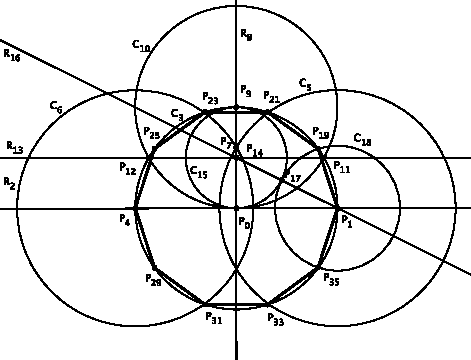
\includegraphics{3_decagon}} 
%\includegraphics{Decagono} 
\caption{Costruzione del decagono}
\end{center}
\end{figure}

\end{frame}



%%%%%%%%%%%%%%%%%%%%%%%%%%%%%%%%%%%%%%%
%%% 3.6) costruzioni euclidee definizioni %%%%%%%%%%%%%%%%%%%%
\begin{frame}
\frametitle{Estensioni ciclotomiche: costruzione dell'eptadecagono}

%%%%%%%%% IMMAGINE COSTRUZIONE EPTADECAGONO %
\begin{figure}[!h]
%centrare
\begin{center}
\resizebox{8.5 cm}{6.3 cm}{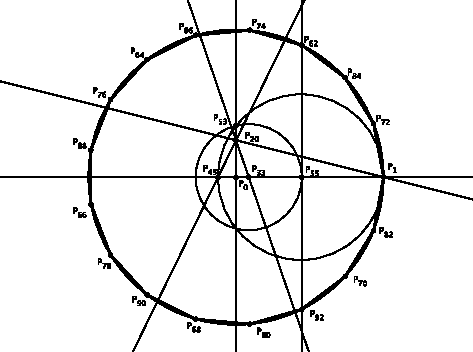
\includegraphics{3_eptadecagon}} 
%\includegraphics{Decagono} 
\caption{Costruzione dell'eptadecagono}
\end{center}
\end{figure}

\end{frame}


%%%%%%%%%%%%%%%%%%%%%%%%%%%%%%%%%%%%%%%%%
%%%%%%%%%%%%%%%%%%%%%%%%%%%%%%%%%%%%%%%%%
%%%%%%%%%%%%%%%%%%%%%%%%%%%%%%%%%%%%%%%%%
%%% 4) Intro capitolo %%%%%%%%%%%%%%%%%%%%%%%%%%%%

\begin{frame}
\begin{center}
Capitolo 4 \\
TRE PROBLEMI IMPOSSIBILI
\end{center}
\end{frame}


%%%%%%%%%%%%%%%%%%%%%%%%%%%%%%%%%%%%%%%
%%% 4.1)  %%%%%%%%%%%%%%%%%%%%
\begin{frame}
\frametitle{Tre problemi impossibili: duplicazione del cubo}

Dato un cubo di lato $1$, per costruirne uno di volume doppio di lato $L$, si deve tracciare un segmento che soddisfi la seguente equazione

\begin{align*}
L^3 = 2 \quad \Rightarrow \quad L = \sqrt[3]{2}
\end{align*}

Questo implica che $L$ soddisfa il polinomio $x^3 - 2$ irriducibile su $\mathbb{Q}$. Ma il grado dell'estensione $\mathbb{Q}(\sqrt[3]{2})$ è $3$, quindi il lato $L$ non è costruibile.
\end{frame}


%%%%%%%%%%%%%%%%%%%%%%%%%%%%%%%%%%%%%%
%% 4.2) %%%%%%%%%%%%%%%%%%%%
\begin{frame}
\frametitle{Tre problemi impossibili: trisezione dell'angolo}

Sia $\alpha = 3\theta = \pi / 3$; costruire l'angolo di $\theta = \pi / 9$ equivale a costruire $cos(\pi / 9)$. 
Dalle note relazioni trigonometriche si ottiene
\begin{align*}
cos(3\theta) = 4 cos^3(\theta) - 3 cos(\theta)
\end{align*}
Da cui per $3\theta = \pi / 3$, si ha che
\begin{align*}
1/2 = 4 cos^3(\pi / 9) - 3 cos(\pi / 9)
\end{align*}
Quindi $cos(\pi / 9)$ soddisfa l'equazione polinomiale
\begin{align*}
8x^3 - 6x - 1 = 0 
\end{align*}

\noindent
irriducibile su $\mathbb{Q}$, di grado $3$. Quindi  $cos(\pi / 9)$ non è costruibile.

\end{frame}



%%%%%%%%%%%%%%%%%%%%%%%%%%%%%%%%%%%%%%%%
%%%% 4.3)  %%%%%%%%%%%%%%%%%%%%
%\begin{frame}
%\frametitle{Tre problemi impossibili: trascendenza di $\pi$}

%Charles Hermite (Dieuze, 1822 - Parigi, 1901) nel tentativo di dimostrare la trascendenza di $\pi$, giunse nel 1873 a dimostrare la trascendenza del numero di Nepero.
%Dopo questo risultato scrisse in una lettera indirizzata al collega tedesco Carl Wilhelm Brochardt le seguenti parole:

%\begin{center}
%\emph{ \lq\lq Non oso tentare di dimostrare la trascendenza di $\pi$. Se altri ci riusciranno, nessuno sarà più felice di me per il loro successo, ma credimi, caro amico, ciò non mancherà di costare loro qualche sforzo.\rq\rq }
%\end{center}

%\end{frame}


%%%%%%%%%%%%%%%%%%%%%%%%%%%%%%%%%%%%%%%
%%% 4.4)  %%%%%%%%%%%%%%%%%%%%
\begin{frame}
\frametitle{Tre problemi impossibili: trascendenza di $\pi$}


Carl Louis Ferdinand von Lindemann (Hannover, 1852 - Gottinga, 1939) nel 1882 scoprì la trascendenza di $\pi$. \\ Inizialmente dimostrò che se $x_1, x_2, \dots, x_n$ sono numeri algebrici distinti, reali o complessi e se $p_1, p_2, \dots, p_n$ sono numeri algebrici non tutti nulli, allora la somma
\begin{align*}
p_1 e^{x_1} + p_2 e^{x_2} + \cdots + p_n e^{x_n}  
\end{align*}
\noindent
è sempre diversa da zero. Per $n = 2$, $p_1 = p_2 = 1$ e $x_2 = 0$ si ha 
\begin{align*}
e^{x_1} + 1 \neq 0  
\end{align*}
\noindent
per ogni $x_1$ algebrico. Ma per la formula di Eulero $e^{i\pi} + 1 = 0$ si ha che $i\pi$ deve essere trascendente, e dato che $i$ è algebrico, si ha che $\pi$ è trascendente.
\end{frame}

%

%%%%%%%%%%%%%%%%%%%%%%%%%%%%%%%%%%%%%%%
%%% 4.5)  %%%%%%%%%%%%%%%%%%%%
\begin{frame}
\frametitle{Tre problemi impossibili: quadratura del cerchio e rettificazione della circonferenza}

$\bullet$ Risolvere il problema della quadratura del cerchio equivale a costruire un quadrato di area uguale a quella di un cerchio assegnato di area $1$. Si deve quindi costruire un segmento di lunghezza $\sqrt{\pi}$ ma tale numero non appartiene a nessun ampliamento di $\mathbb{Q}$ avente grado una potenza di due.
\\
$\bullet$ Risolvere il problema della rettificazione della circonferenza equivale a costruire un segmento di lunghezza uguale alla lunghezza di una circonferenza di raggio unitario. Si deve quindi costruire un segmento di lunghezza $2\pi$. Ma come nel caso precedente $2\pi$ non è costruibile in virtù della trascendenza di $\pi$.

\end{frame}




%%%%%%%%%%%%%%%%%%%%%%%%%%%%%%%%%%%%%%%
%%%%%%%%%%%%%% BIBLIOGRAFIA  %%%%%%%%%%%%%%%%%%%%%%%%%%%
%%%%%%%%%%%%%%%%%%%%%%%%%%%%%%%%%%%%%%%%%%%%%%%%%
\begin{frame}
\frametitle{Bibliografia essenziale}
\begin{thebibliography}{12}


\bibitem{Artin}
Michael Artin, \emph{Algebra}, Prentice Hall of India, New Delhi 2007 

\bibitem{kline}
Morris Kline \emph{Storia del pensiero matematico, dal settecento ad oggi}, volume secondo, Einaudi editore 1991.

\bibitem{Kosh}
Thomas Koshy, \emph{Elementary Number Theory with applications}, Accademic Press, Elzevier, 2007.

\bibitem{Livio}
Mario Livio, \emph{L'equazione impossibile}, ed. BUR 2007.

\bibitem{cattaneo}
Giulia Maria Piacentini Cattaneo, \emph{Algebra, un approccio algoritmico}, Zanichelli 2007, prima ed. 1996.

\bibitem{Procesi}
Claudio Procesi, \emph{Elementi di teoria di Galois}, Zanichelli 2008.

\bibitem{Rogg}
Margherita Roggero, \emph{Appunti ed esercizi di Matematica Discreta}, Quaderni didattici dell'Università di Torino, 2005.

\bibitem{Stewart}
Ian Stewart, \emph{Galois Theory}, Chapman and Hall 1973, prima ed. 2006.

\end{thebibliography}


\end{frame}




\end{document}




%%%%%%%%%%%%%% BIBLIOGRAFIA  %%%%%%%%%%%%%%%%%%%%%%%%%%%
%%%%%%%%%%%%%%%%%%%%%%%%%%%%%%%%%%%%%%%%%%%%%%%%%
%\newpage

%\begin{thebibliography}{10}

%\bibitem{Artin}
%Michael Artin, \emph{Algebra}, Prentice Hall of India, New Delhi 2007 

%\bibitem{Baker}
%Alan Baker, \emph{Transcendental Number theory}, Cambridge univesity press 1990, prima ed. 1975.

%\bibitem{Dante}
%Dante Alighieri, \emph{La Divina Commedia}, Einaudi 1954.

%\bibitem{Boyer}
%Carl B. Boyer, \emph{Storia della matematica}, Mondadori 2005, prima ed. 1976.

%\bibitem{kline}
%Morris Kline \emph{Storia del pensiero matematico, dal settecento ad oggi}, volume secondo, Einaudi editore 1991.

%\bibitem{Kosh}
%Thomas Koshy, \emph{Elementary Number Theory with applications}, Accademic Press, Elzevier, 2007.

%\bibitem{Livio}
%Mario Livio, \emph{L'equazione impossibile}, BUR 2007, prima ed. 2006.

%\bibitem{Shea}
%Donald O'Shea, \emph{La congettura di Poincarè}, BUR, Milano 2007.

%\bibitem{cattaneo}
%Giulia Maria Piacentini Cattaneo, \emph{Algebra, un approccio algoritmico}, Zanichelli 2007, prima ed. 1996.

%\bibitem{Plato}
%Platone, \emph{Dialoghi}.

%\bibitem{Procesi}
%Claudio Procesi, \emph{Elementi di teoria di Galois}, Zanichelli 2008, prima ed. 1977.

%\bibitem{Rogg}
%Margherita Roggero, \emph{Appunti ed esercizi di Matematica Discreta}, Quaderni didattici dell'Università di Torino, 2005.

%\bibitem{Russo}
%Lucio Russo, \emph{La rivoluzione dimenticata: il pensiero scientifico greco e la scienza moderna}, Feltrinelli Milano 1997.

%\bibitem{Shanks} 
%Daniel Shanks \emph{Solved and unsolved problems in Number Theory }, AMS 1993, prima ed. 1962

%\bibitem{Stewart}
%Ian Stewart, \emph{Galois Theory}, Chapman and Hall 1973, prima ed. 2006.

%\bibitem{sitowolfram}
%Dal Web: sito della Wolfram Research, pagina sulla costruzione dell'eptadecagono:  \begin{verbatim} http://mathworld.wolfram.com/Heptadecagon.html \end{verbatim}

%\bibitem{sitoroi}
%Dal Web: sito del prof. Lorenzo Roi, pagina sulla costruzione del decagono e dell'eptadecagono: \begin{verbatim} http://www.lorenzoroi.net/geometria/Poligoni.html \end{verbatim}

%\bibitem{sito3}
%Da Wikipedia, sulla trisezione dell'angolo: \begin{verbatim} http://it.wikipedia.org/wiki/Trisezione_dell'angolo \end{verbatim}

%\bibitem{sito2}
%Da Wikipedia, sul problema di Delo: \begin{verbatim} http://it.wikipedia.org/wiki/Problema_di_Delo \end{verbatim}

%\bibitem{sito2}
%Da Wikipedia, sulla quadratura del cerchio: \begin{verbatim} http://it.wikipedia.org/wiki/Quadratura_del_cerchio \end{verbatim}

%\bibitem{sito4}
%Da Wikipedia, sulla costruzione dell'eptadecagono: \begin{verbatim} http://it.wikipedia.org/wiki/Eptadecagono \end{verbatim}

%\end{thebibliography}


%%% asterix

%%%%%%%%%%%%%%%%%%%%%%%%%%%%%%%%%%%%%%%%%
%%%% 1.8) costruzioni radice quadrata I%%%%%%%%%%%%%%%%%
%\begin{frame}
%\frametitle{Costruzioni Euclidee: radice quadrata di un segmento I}
%A titolo di esempio si propone la costruzione di $\sqrt{\alpha}$, dove $P_{0}P_{1} = 1$ e $P_{0}P_{10} = \alpha$ è il segmento dato.

%%%%%%%%% IMMAGINE COSTRUZIONE PARALLELE %
%\begin{figure}[!h]
%%centrare
%\begin{center}
%\resizebox{8.5 cm}{6.3 cm}{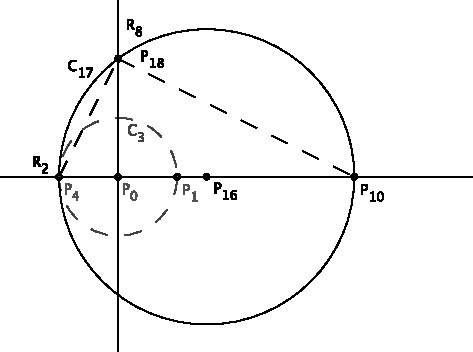
\includegraphics{1_Es7_radice}} 
%%\includegraphics{Es1perpendicolare} 
%\caption{Costruzione di $\sqrt{\alpha}$}
%\end{center}
%\end{figure}
%\end{frame}

%
%%%%%%%%%%%%%%%%%%%%%%%%%%%%%%%%%%%%%%%%%%
%%%% 
%\begin{frame}
%\frametitle{Costruzioni Euclidee: radice quadrata di un segmento II}
%La costruzione euclidea del procedimento appena descritto è data da:
%\begin{align*}
%S_{6} = ( &P_{0}, P_{1}, R_{2}(P_{0}, P_{1}), C_{3}(P_{0};\overline{P_{0} P_{1}}), \\
%&P_{4}(C_{3}, R_{2} ), C_{5}(P_{1};\overline{P_{1} P_{4}}), C_{6}(P_{4};\overline{P_{1} P_{4}}),\\
%&P_{7}(C_{5}, C_{6} ), R_{8}(P_{0}, P_{7}), C_{9}(P_{0}; \alpha ), P_{10}(C_{9}, R_{2} ) \\
%&C_{11}(P_{4}, \overline{P_{4} P_{10}}) ), C_{12}(P_{10}, \overline{P_{10} P_{4}}), \\
%&P_{13}(C_{11},C_{12}), P_{14}(C_{11},C_{12}),   R_{15}(P_{13}, P_{14}), \\
%&P_{16}(R_{2},R_{15}) ), C_{17}(P_{16};\overline{P_{16} P_{10}}), P_{18}(C_{17}, R_{8} ) )
%\end{align*}
%\end{frame}


%%%%%%%%%%%%%%%%%%%%%%%%%%%%%%%%%%%%%%%
%%% 2.1) costruzioni euclidee definizioni %%%%%%%%%%%%%%%%%%%%
%\begin{frame}
%\frametitle{Numeri euclidei: definizioni I}

%\begin{definizione}
%L'insieme delle possibili costruzioni euclidee, aventi $P_0$ e $P_1$ come punti iniziali, indicato con $\mathcal{E}(P_0,P_1)$, può essere immerso nel piano $\mathbb{R}\times\mathbb{R}$, definendo la seguente funzione:
%\begin{align*} 
%\mathcal{I}:  \mathcal{E}(P_0,P_1) & \longrightarrow \mathbb{R}\times\mathbb{R} \\
%P_0 & \longmapsto (0,0) \\
%P_1 & \longmapsto (1,0) \\
%\end{align*}
%L'immagine di tale funzione è chiamata insieme delle \begin{bfseries}costruzioni euclidee nel piano reale\end{bfseries} e indicata con  $\mathcal{E}_{\mathbb{R}\times\mathbb{R}}$.
%\end{definizione}

%Si ottiene così una biiezione fra i punti, le rette e le circonferenze  delle costruzioni euclidee con quelle sul piano reale.

%\end{frame}




%%%%%%%%%%%%%%%%%%%%%%%%%%%%%%%%%%%%%%%%
%%%% 1.2) costruzioni euclidee definizioni %%%%%%%%%%%%%%%%%%%%
%\begin{frame}
%\frametitle{Estensioni ciclotomiche: numeri di Fermat}
%\begin{center}
%I numeri del tipo $F_n = 2^{2^{n}} +1$, che in questo contesto assumono un'importanza particolare, sono detti numeri di Fermat. 
%\end{center}
%\begin{align*}
%F_0 &= 3 &F_3 &= 257\\
%F_1 &= 5 &F_4 &= 65537\\
%F_2 &= 17 &F_5 &= 4294967297 
%%\end{align*}
%%\begin{align*}  
%%F_5 &= 2^{2^{5}} + 1 = 4294967297 = 641 \cdot 6700417
%\end{align*}
%\begin{teorema}
%Sia $F_n$ l'$n$-esimo numero di Fermat, allora, $F_n = F_{n-1}^2 - 2F_{n-1} + 2$ per $n \geq 1$.
%\end{teorema}
%\end{frame}

%%%%%%%%%%%%%%%%%%%%%%%%%%%%%%%%%%%%%%%%%
%%%%% 1.2) costruzioni euclidee definizioni %%%%%%%%%%%%%%%%%%%%
%\begin{frame}
%\frametitle{Estensioni ciclotomiche: costruzione del decagono II}

%La costruzione euclidea del procedimento appena descritto è data da:
%\begin{align*}
%S_{d} =  &P_{0}, P_{1}, R_{2}(P_{0}, P_{1}), C_{3}(P_{0};\overline{P_{0} P_{1}}), P_{4}(C_{3}, R_{2} ), C_{5}(P_{1};\overline{P_{1} P_{4}}),\\
%&C_{6}(P_{4};\overline{P_{1} P_{4}}), P_{7}(C_{5}, C_{6} ), R_{8}(P_{0}, P_{7}), P_{9}(C_{3}, R_{8}),  C_{10}(P_{9};\overline{P_{9} P_{0}}), \\
%&P_{11}(C_{3}, C_{10}), P_{12}(C_{3}, C_{10}), R_{13}(P_{11}, P_{12}), P_{14}(R_{8}, R_{13})), \\
%& C_{15}(P_{14};\overline{P_{14} P_{0}}), R_{16}(P_{1}, P_{14}), P_{17}(C_{15}, R_{16}), C_{18}(P_{1};\overline{P_{1} P_{17}}), \\
%&P_{19}(C_{3},C_{18}), C_{20}(P_{19};\overline{P_{19} P_{1}}), P_{21}(C_{3}, C_{20}), C_{22}(P_{21};\overline{P_{21} P_{19}}),  \\
%&P_{23}(C_{3}, C_{22}), C_{24}(P_{23};\overline{P_{23} P_{21}}), P_{25}(C_{3}, C_{24}), C_{26}(P_{25};\overline{P_{25} P_{23}}), \\
%&P_{27}(C_{3}, C_{26}), C_{28}(P_{27};\overline{P_{27} P_{25}}), P_{29}(C_{3}, C_{28}), C_{30}(P_{29};\overline{P_{29} P_{27}}), \\
%&P_{31}(C_{3}, C_{30}), C_{32}(P_{31};\overline{P_{31} P_{29}}), P_{33}(C_{3}, C_{32}), C_{34}(P_{33};\overline{P_{33} P_{31}}), \\
%& P_{35}(C_{3}, C_{34}))
%\end{align*}

%\end{frame}


%\begin{osservazione} 
%L'insieme di punti $\mathbb{Z}\times \mathbb{Z} := \{(m,n) \mid m \in \mathbb{Z}, n \in \mathbb{Z}\}$ è un sottoinsieme di $E$. A partire dai punti iniziali $P_0$ e $P_1$ è sempre possibile costruire un sistema di assi cartesiani ortogonali, i cui punti vanno a ricalcare $\mathbb{Z}\times \mathbb{Z}$ nelle costruzioni euclidee nel piano reale.
%\end{osservazione}

%\begin{osservazione} 
%L'insieme di punti $\mathbb{Q} := \{ \frac{m}{n} \mid m \in \mathbb{Z}, n \in \mathbb{Z} - \emptyset \}$ è un sottoinsieme di $E$.
%\end{osservazione}

%\end{frame}

%
%%%%%%%%%%%%%%%%%%%%%%%%%%%%%%%%%%%%%%%%
%%%% 2.2) costruzioni euclidee definizioni %%%%%%%%%%%%%%%%%%%%
%\begin{frame}
%\frametitle{Numeri euclidei: definizioni II}



%\begin{osservazione}
%Si osserva che un punto è euclideo se e solo se lo sono le sue rispettive coordinate nel piano reale.
%\end{osservazione}
